\section{Aufgabe 1: Entscheidungsbäume}
\subsection{Feature Engineering}

\subsection{Analyse der Zielvariable}
%TODO: Vll nicht der beste Einstieg?}
Wie Abbildung \ref{fig:disc_target_variable} entnommen werden kann ist Ausprägung der Zielvariable ungleich auf beide Klassen verteilt. Die Klassifizierungsgenauigkeit eines Modells muss demnach unter Berücksichtigung der sogenannten \emph{Null Accuracy} bewertet werden. Unter \emph{Null Accuracy} versteht man die Genauigkeit eines Modells, dass unabhängig von allen Eingaben immer die am häufigsten auftretende Klasse vorhersagt. In unserem Fall würde ein Modell, welches immer Regen vorhersagt, eine Klassifizierungsgenauigkeit von 79,39\% erreichen. Das Ziel der nachfolgenden Schritte ist also ein Modell mit einer besseren Klassifizierungsgenauigkeit als die \emph{Null Accuracy} aufzubauen.

\begin{figure}[h]
	\centering
	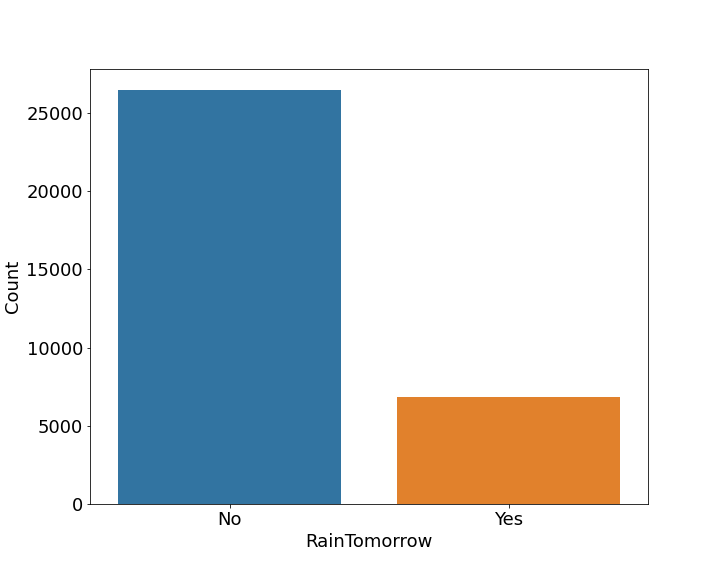
\includegraphics[width = 0.5\textwidth]{Bilder/distribution_target_variable}
	\caption{Verteilung der Zielvariable}
	\label{fig:disc_target_variable}
\end{figure}

\subsubsection{Fehlende Werte}
%TODO: Gesamter Absatz noch super holprig
Der zu untersuchende Datensatz beinhaltet fehlende Werte. Diese müssen für eine weitere Verarbeitung bereinigt werden. Im Folgenden werden Methoden beschrieben, wie mit den fehlenden Werte umgegangen wurde:
\begin{description}
	\item[Fehlende Zielvariable]\hfill \\
	 Im ersten Schritt wurden 834 Beobachtungen, welche keinen Wert für die Zielvariable \emph{RainTomorrow} aufweisen, aus dem Datensatz entfernt. Damit wurde die Anzahl an Beobachtungen auf 33402 reduziert.
	 \item[Spalten mit fehlenden Werten]\hfill \\
	 In einem nächsten Schritt werden die Spalten aus dem Datensatz entfernt, in denen mehr als 40\% der beinhaltenden Variablen fehlen. Namentlich wurden somit die Spalten \emph{Evaporation, Sunshine, Cloud9am} sowie \emph{Cloud3pm} aus dem Datensatz entfernt. Der Schwellwert von 40\% wurde empirisch festgelegt und hat zu den besten Klassifizierungsergebnissen geführt.
	 \item[Beobachtungen mit fehlenden Werten]\hfill \\
	 Des Weiteren werden Beobachtungen aus dem Datensatz entfernt, von denen mehr als 50\% der Variablen fehlen. Durch diesem Schritt wurden 55 Beobachtungen aus dem Datensatz entfernt.
	 \item[Imputation]\hfill \\
	 Durch die zuvor beschriebenen Methoden ist der Datensatz noch immer nicht frei von fehlenden Werten. Um diese zu ersetzen werden für kategorische und numerische Variablen verschiedene Strategien zur Imputation verfolgt. Fehlende numerische Werte werden mit dem Median der jeweiligen Variable ersetzt. Der Median wurde gewählt, da dieser im Vergleich zum Mittelwert robuster gegenüber Ausreißern ist. Für kategorielle Variablen hingegen wird der am häufigsten vorkommende Wert verwendet. Wichtig bei der Ermittlung des Medians bzw. des häufigsten Wertes ist, dass dieser ausschließlich mit Hilfe der Trainingsdaten ermittelt wird. Es muss davon ausgegangen werden, dass die Testdaten nicht bekannt sind. Die Ermittlung auf Basis des gesamten Datensatzes, inklusive der Testdaten, würde zu \emph{Data-Leakage} führen und ist zu vermeiden. Die auf Basis der Trainingsdaten ermittelten Werte für die Imputation werden auf die Trainings- und Testdaten angewendet.
\end{description}


\subsubsection{Merkmalsaufteilung}
Das Feld \emph{Datum} wurde in die Merkmale \emph{Year, Month} und \emph{Day} aufgeteilt.

\subsubsection{Merkmalserstellung}
Eine weit verbreitete Technik des Feature Engineerings ist die Erstellung zusätzlicher Merkmalen. Somit wurde die Variable \emph{MinMaxDiff} erstellt, welche die Differenz zwischen der minimalen und der maximalen Tages-Temperatur angibt. In gleicher Weise wurden die Variablen \emph{PressureDiff, HumidityDiff und WindSpeedDiff} erstellt.

\subsubsection{Diskretisierung}
Die Diskretisierung eines Merkmals kann eine Überanpassung bei der Erstellung von Modellen verhindern, indem der Wertebereich des Merkmals minimiert und somit generalisiert wird. Es sollte beachtet werden, dass der Informationsverlust durch die Diskretisierung nicht zu hoch ausfällt.\\
\noindent \hspace*{7mm}
Zu Testzwecken wird das neu erstellte Merkmal \emph{Month} in zwei weiteren Merkmalen diskretisiert. Zum einen wird das kategorische Merkmal \emph{Season} erstellt, welches angibt,  in welcher Jahreszeit der Monat liegt. Zum anderen gibt das Boolean Merkmal \emph{RainyMonth} an, ob es sich um einen in Erwartung regenreichen Monat handelt.

\subsubsection{Kodierung kategorischer Werte}
Um kategorische Werte für weitere Analysen verwenden zu können, müssen diese in numerische Werte umkodiert werden. Hierbei wurden die folgenden Strategien Angewendet:
\begin{description}
	\item[Binäre Kodierung]\hfill \\
	%TODO: Das hört sich hoprig an.
	Die Zielvariable \emph{RainTomorrow}, sowie die Variable \emph{RainToday} liegen mit den binären Ausprägungen \emph{Yes} und \emph{No} vor. Die binären Werte wurden in eine numerische Darstellung umgewandelt
	\item[One-Hot-Kodierung]\hfill \\ 
	%TODO: auch sholprig
	Das neu diskretisierte Merkmal \emph{Season} wird mittels \emph{One-Hot Encoding} in drei Boolean Spalten aufgeteilt. Eine einfache Zuteilung eines Zahlenwertes pro auftretender Variablenausprägung hat den Nachteil, dass dadurch eine metrische numerische Variable für ein gegebenenfalls nicht metrisch interpretierbares Merkmal entsteht. Für Entscheidungsbäume wäre dies kein Problem, jedoch sollte das Feature Engineering weitgehend unabhängig von dem verwendeten Klassifizierungsalgorithmus durchgeführt werden.
	\item[Ziel-Kodierung]\hfill \\ 
	%TODO: Deutsch oder Englisch? Bedingte Wsl. vll als Mathematische schreibweise? 
	Mit Hilfe des \emph{Target Encodings} werden die Merkmale \emph{Location, WindGustDir, WindDir9am} und \emph{WindDir3pm} verarbeitet. Dabei werden den jeweiligen Merkmalsausprägungen ihr Einfluss auf die Zielvariable zugeordent, also die bedingte Wahrscheinlichkeit, dass unter der Bedingung, dass z.B. Merkmal \emph{Location} für die Zielvariable (\emph{Target}) den Wert 1 (in unsrem Fall "Yes") annimmt. Zum Beispiel wird die Merkmalsausprägung "Perth" mit dem Wert 0.2 kodiert, wenn 20\% der jeweiligen Beobachtungen für die Zielvariable den Wert "Yes"  annehmen.  Somit wird keine zufällige Zuteilung von nummerischen Werten verteilt, sondern direkt einen Verbindung zu Zielvariable hergestellt. Ein Nachteil des Target Encoding ist, dass genau durch diese Verbindung zur Zielvariable die Wahrscheinlichkeit des Overfittings steigt (vgl. https://towardsdatascience.com/why-you-should-try-mean-encoding-17057262cd0   keine Wissenschaftliche Quelle).
\end{description}

\subsubsection{Bereinigung von Ausreißern}
Ausreißer können die Performance eines Modells mindern, indem sie als Hebelwerte agieren und somit die Schätzungen der Zielvariable verzerren. Aus diesem Grund werden die Merkmale des Datensatz hinsichtlich ihrer Ausreißer begutachtet. Es wird ersichtlich, dass nur die Merkmale \emph{Rainfall} und \emph{WindGustSpeed} abweichende Werte aufweisen. Das Enfernen dieser Werte aus dem Datensatz führt jedoch zu einer schlechteren Performance der im folgenden Abschnitt besprochenen Entscheidungsbäume. Deshalb werden die Beobachtungen nicht aus dem Datensatz entfernt. Zudem zählen die beiden Merkmale zu denjenige Merkmalen, die durch die Variablenselektion aussortiert und somit für weitere Modelle nicht mehr betrachtet werden.

\subsubsection{Variablenselektion}
Nach dem durchgeführten Feature Engineering verfügt der Datensatz über 28 Einflussvariablen. Durch eine Variablenselektion wird diese Anzahl verringert. Das hat den Vorteil, dass Modelle besser interpretierbar sind. Zudem steigert es die Performance von Modellen, indem nicht relevante Merkmale ausgeschlossen werden, wodurch auch die Wahrscheinlichkeit des Overfittings sinkt.\\
\noindent \hspace*{7mm}
Für den betrachteten Datensatz wird eine univariate Variablenselektion mit dem Modul \emph{SelectKBest} der Bibliothek \emph{sklearn} durchgeführt. Dabei werden die \textit{k=5} Merkmale ausgewählt, die den höchsten Wert der F-Statistik aufweisen. Dieser Wert gibt an, ob ein einzelnes Merkmal eine signifikante Verbesserung des Modells erzielt. Dazu wird ein Modell ohne dieser Variable mit einem Modell mit der beobachteten Variable verglichen. Als Ergebnis wurden  die Merkmale \emph{WindGustDir, Humidity9am, Humidity3pm, RainToday} und \emph{MinMaxDiff} ausgewählt.

\vspace{1cm}
\subsection{Entscheidungsbäume}
%TODO: Quellen! Tobi
Für die Erstelltung der Entscheidungsbäume wurde der Datensatz in eine Trainings- und eine Testmenge eingeteilt. Dabei beträgt das Verhältnis 8:2. 80\% der Daten sind genügend, um ein gutes Modell zu trainieren. 20\% sind eine ausreichende Menge, um einen genauen Testfehler und die Modellgüte zu bestimmen.
\subsubsection{Default-Einstellungen}
Quelle: https://scikit-learn.org/stable/modules/generated/sklearn.tree.DecisionTreeClassifier.html\\
Die Entscheidungsbäume werden mit dem Modul \emph{tree.DecistionTreeClassifier} erstellt. Im ersten Aufgabenteil werden dazu die Default-Einstellungen des Moduls genutzt.\\
\noindent \hspace*{7mm}
Diese geben an, dass ein Baum immer maximal gebaut wird (\emph{max\_depth = None}). Das heißt, so lange mehr als ein Objekt in einem Knoten vorliegt, wird dieser Knoten weiter aufgespalten (\emph{min\_samples\_split = 2}). Das Ergebnis ist überangepasst, da jeder einzelne Datenpunkt ein eigenes Blatt im Baum bekommt (\emph{min\_samples\_leaf = 1}). Dieser Baum kann somit nicht auf unbekannte Daten generalisiert werden und der Testfehler fällt sehr hoch aus. Die Splits werden mit dem Gini-Wert durchgeführt und nicht mit der Entropie (\emph{citerion=\gqq{gini}}). Zudem werden für jedes Spalten alle Merkmale einbezogen, um den besten \emph{Split} zu finden (\emph{max\_features = None}). In Abbildung \ref{fig:treedefault} wird der mit den Default-Einstellungen erzeugte Baum dargestellt.
\begin{figure}[h]
	\centering
	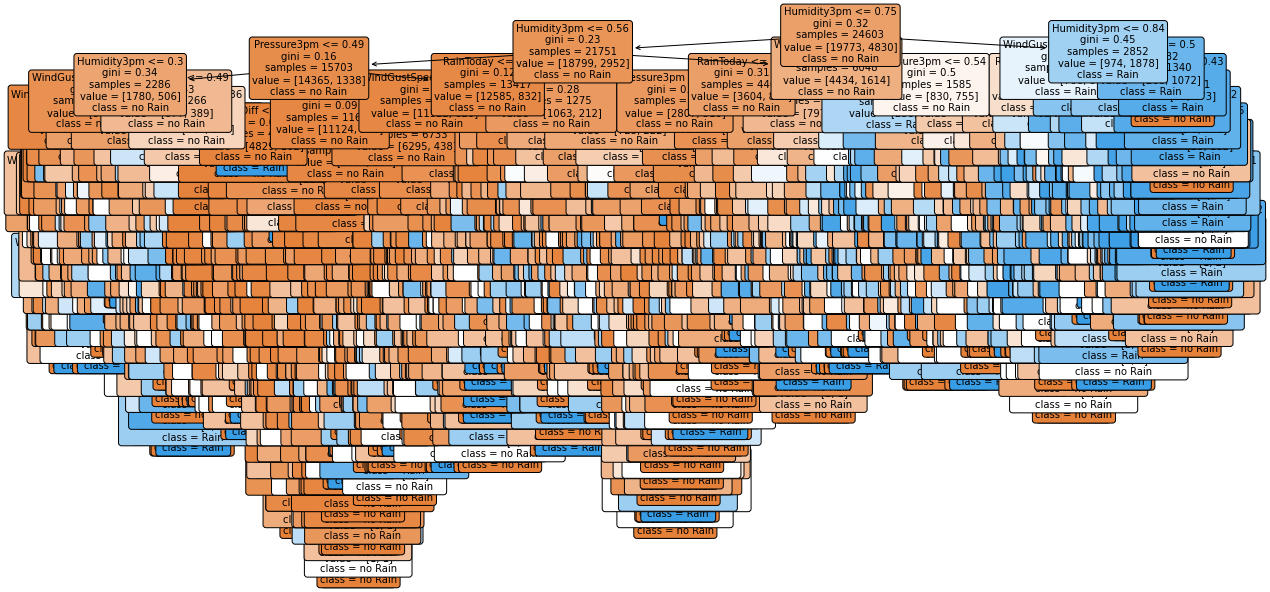
\includegraphics[width = 0.7\textwidth]{Bilder/treedefault}
	\caption{Entschidungsbaum mit Default-Einstellungen}
	\label{fig:treedefault}
\end{figure}
Es ist leicht zu erkennen, dass dieser Baum zu viele Knoten und Blätter enthält und somit eine Überanpassung darstellt. Diese Überanpassung kann auch an dem Trainings- und Testfehler abgelesen werden. Der Trainingsfehler beträgt für den gebildeten Entscheidungsbaum 0.0005 und der Testfehler 0.2340. Der Testfehler ist damit höher als bei einem Modell, das zufällig entscheidet. Dem kann mit verschiedenen Einstellungen entgegengewirkt werden.
\subsubsection{Variationen}
%TODO: Beschreibiung einzelner Einstellungen Tamara
Um einen übersichtlichen und brauchbaren Entscheidungsbam erzeugen zu können werden verschiedenen Einstellungen für die Parameter \emph{max\_depth, min\_ipurity\_decrease} und \emph{criterion} angewandt. Im Folgenden werden die Entscheidungsbäume dargestellt, deren Parameter mit Hilfe des \textbf{GridSearch Verfahrens} festgelegt wurden. Bei der Visualisierung liegt der Fokus auf der Struktur des Baumes und nicht darauf, dass die einzelnen Knoten identifiziert werden können.\\
\begin{figure}[H]
    \centering
     \begin{minipage}{0.30\textwidth}
        \centering
        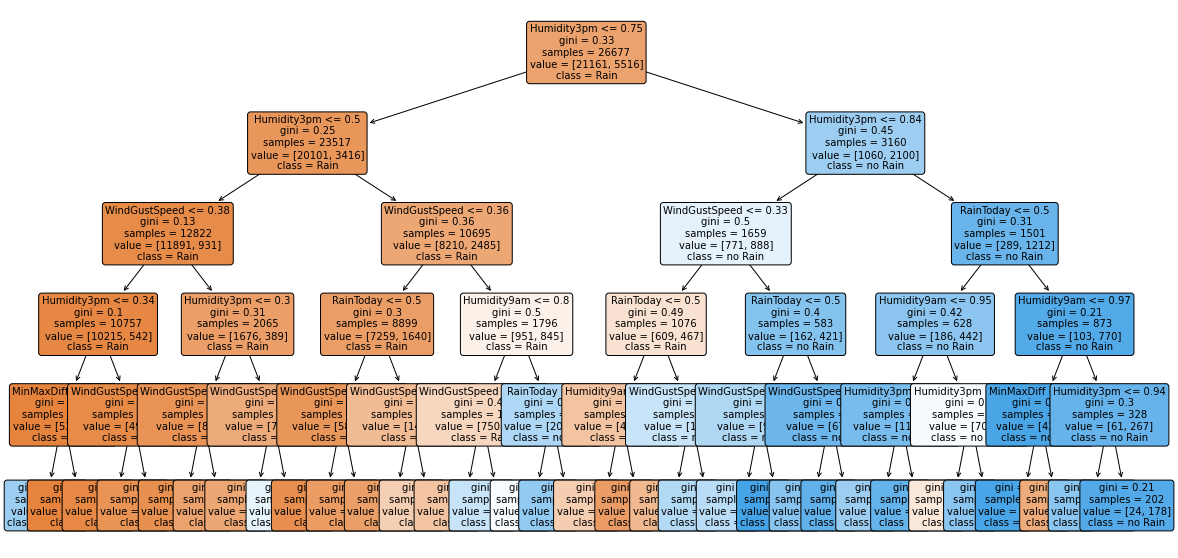
\includegraphics[width=0.9\textwidth]{Bilder/treeMaxDepth} % first figure itself
        \caption{Maximale Tiefe von 5}
        \label{fig:treeMaxDepth}
    \end{minipage}\hfill
    \begin{minipage}{0.30\textwidth}
        \centering
        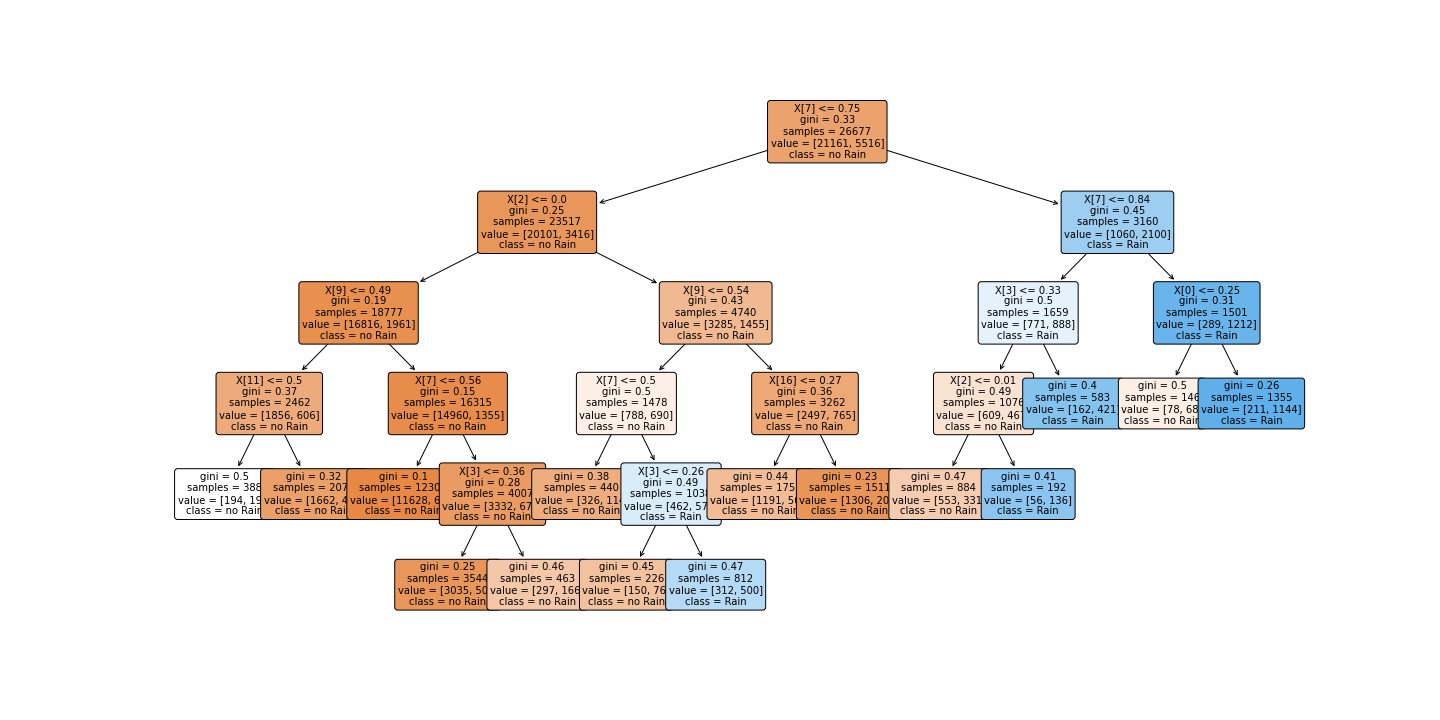
\includegraphics[width=0.9\textwidth]{Bilder/treeMinImpurityDecrease} % first figure itself
        \caption{Minimale Unschärfe Reduktion von 0.003}
        \label{fig:treeMinImpurityDecrease}
    \end{minipage}\hfill
    \begin{minipage}{0.30\textwidth}
        \centering
        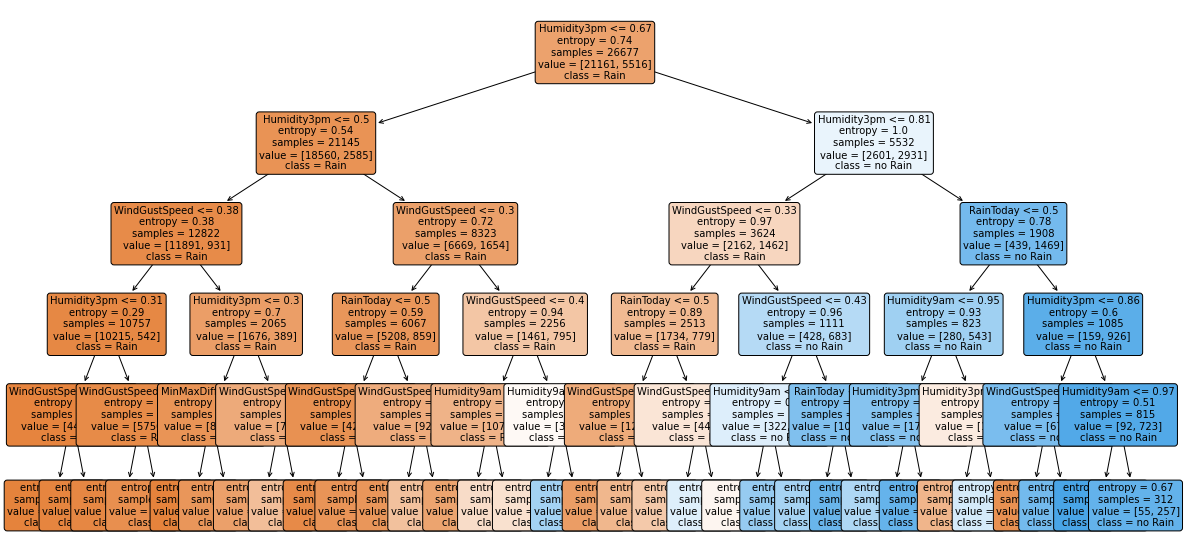
\includegraphics[width=0.9\textwidth]{Bilder/treeCriterion} % second figure itself
        \caption{Entropie als Entscheidungskriterium}
        \label{fig:treeCriterion}
    \end{minipage}
\end{figure}
\begin{description}
	\item[Maximale Tiefe]\hfill \\
	In Abbildung \ref{fig:treeMaxDepth} wurde eine maximale Tiefe von \textbf{fünf} angegeben. Trotz der geringen Tiefe entstehen schon zu viele Blatt Knoten für eine übersichtliche Visualisierung. Im Gegensatz zu den anderen Variationen ist dieser Baum \textbf{symmetrisch}, da jeder Ast bis zur gleichen Tiefe verfolgt wird. Dieser Baum entspricht den ersten fünf Stufen des vorher erstellten Default-Entscheidungsbaum, da der \emph{max\_depth}-Parameter den Baum einfach an der gegebenen Stufe abschneidet.
	\item[Unschärfe-Reduktion]\hfill \\ 
	In Abbildung \ref{fig:treeMinImpurityDecrease} wurde mit dem Parameter \emph{min\_impurity\_decrease} festgelegt, wie viel ein weiterer Knoten die \textbf{Unschärfe} des Entscheidungsbaumes reduzieren muss, um ausgebildet zu werden. Dabei wird jeder zu bildende Knoten einzeln bewertet, sodass es zu einem nicht symmetrischen Baum kommen kann, da nicht jeder Ast bis in die gleiche Tiefe verfolgt wird.
	\item[Entscheidungskriterium]\hfill \\ 
	In Abbildungen \ref{fig:treeCriterion} wurde zusätzlich zur maximalen Tiefe von fünf das Entscheidungskriterium angepasst. Hier wird mit Hilfe der Entropie statt des Gini-Wertes entschieden, welcher Split durchgeführt wird. Die Struktur des Baumes wird dadurch nicht geändert, jedoch können die Knoten voneinander abweichen. Die Entropie erzeugt bei sonst gleich bleibenden Parametern einen Entscheidungsbaum, der einen kleineren Testfehler aufweist.
\end{description}
%TODO Grid Search Tobi
\subsubsection{Minimal Cost-Complexity-Pruning}
%TODO Tamara



